\documentclass[openany]{article} 
\usepackage[english]{babel}
\usepackage[utf8]{inputenc}
\usepackage[T1]{fontenc}
\usepackage{geometry} 
\usepackage{graphicx}
\usepackage{caption}
\usepackage{subcaption}
\usepackage{hyperref}

\hypersetup{
    colorlinks=true,
    linkcolor=blue,
    filecolor=magenta,      
    urlcolor=blue
}

\title{Visual Data Analytics: Practical Exercise}
\date{WS 2022/2023}
\author{Matilde Tozzi}
%\renewcommand{\baselinestretch}{1.1}

\renewcommand{\thesubsection}{\thesection.\alph{subsection}}

\begin{document}

\maketitle

\section {First part: ParaView}

In the first section we use the ParaView software to test a wide range of visualisations.

\subsection {VisHuman Head}

For this task we used the \texttt{vmhead256cubed.raw} file. When opened in ParaView, we need to specify how the data is encoded in the file and this is done by setting the properties according to the \texttt{vmhead256cubed.dat} file, so in this case we had a dataset of 3D 0-255 values of \texttt{unsigned char} format. 

Then, we use a \textit{volume} rendering and we set the transfer function in order to display mostly the bones of the person, keeping the skin just in transparency. This is done by cutting the first peak of density values, that are mostly noise, and also the second peak of density values, that correspond to the majority of flesh. The highest density values, corresponding to the bones, are set to the maximum opacity. We used a modified version of the \textit{X Ray} color map.

\begin{figure}[h]
\centering
\begin{subfigure}{.45\textwidth}
  \centering
  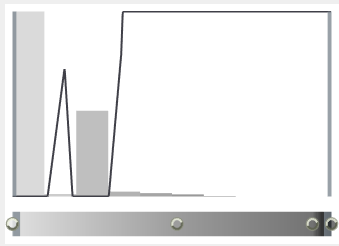
\includegraphics[width=\linewidth]{VisHuman_Head/transfer_function_1}
  \caption{Used transfer function}
\end{subfigure}%
\begin{subfigure}{.5\textwidth}
  \centering
  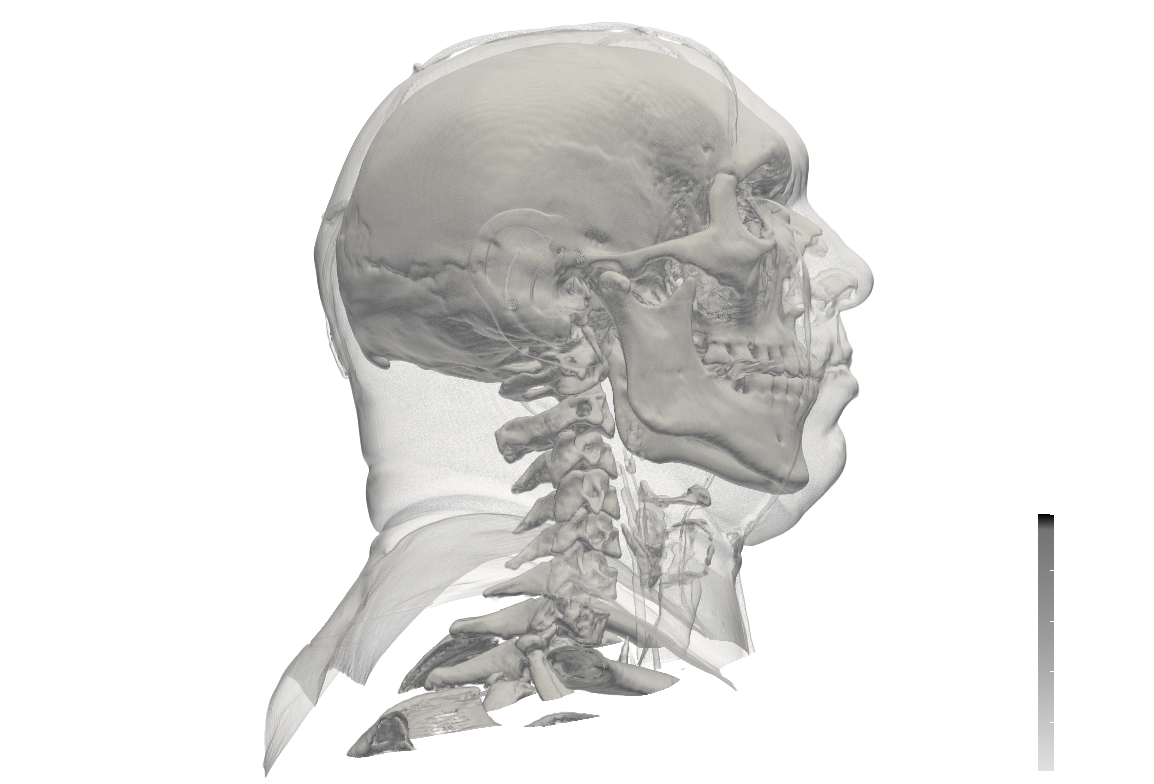
\includegraphics[width=\linewidth]{VisHuman_Head/human_head_1}
  \caption{Resulting visualisation}
\end{subfigure}
\caption{Visualising bones}
\end{figure}

We also tried to expand this concept by using a different color map and a smoother transition to total opacity in order to see which bones have the maximum density. To do so, we used the \textit{Rainbow Uniform} color map. As expected, the most dense bones of the upper part of the body are the teeth.

\begin{figure}[h]
\centering
\begin{subfigure}{.4\textwidth}
  \centering
  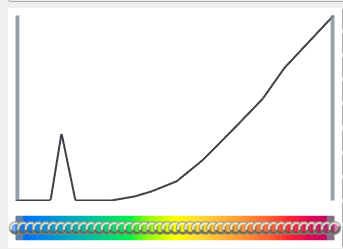
\includegraphics[width=\linewidth]{VisHuman_Head/transfer_function_2}
  \caption{Used transfer function}
\end{subfigure}%
\begin{subfigure}{.6\textwidth}
  \centering
  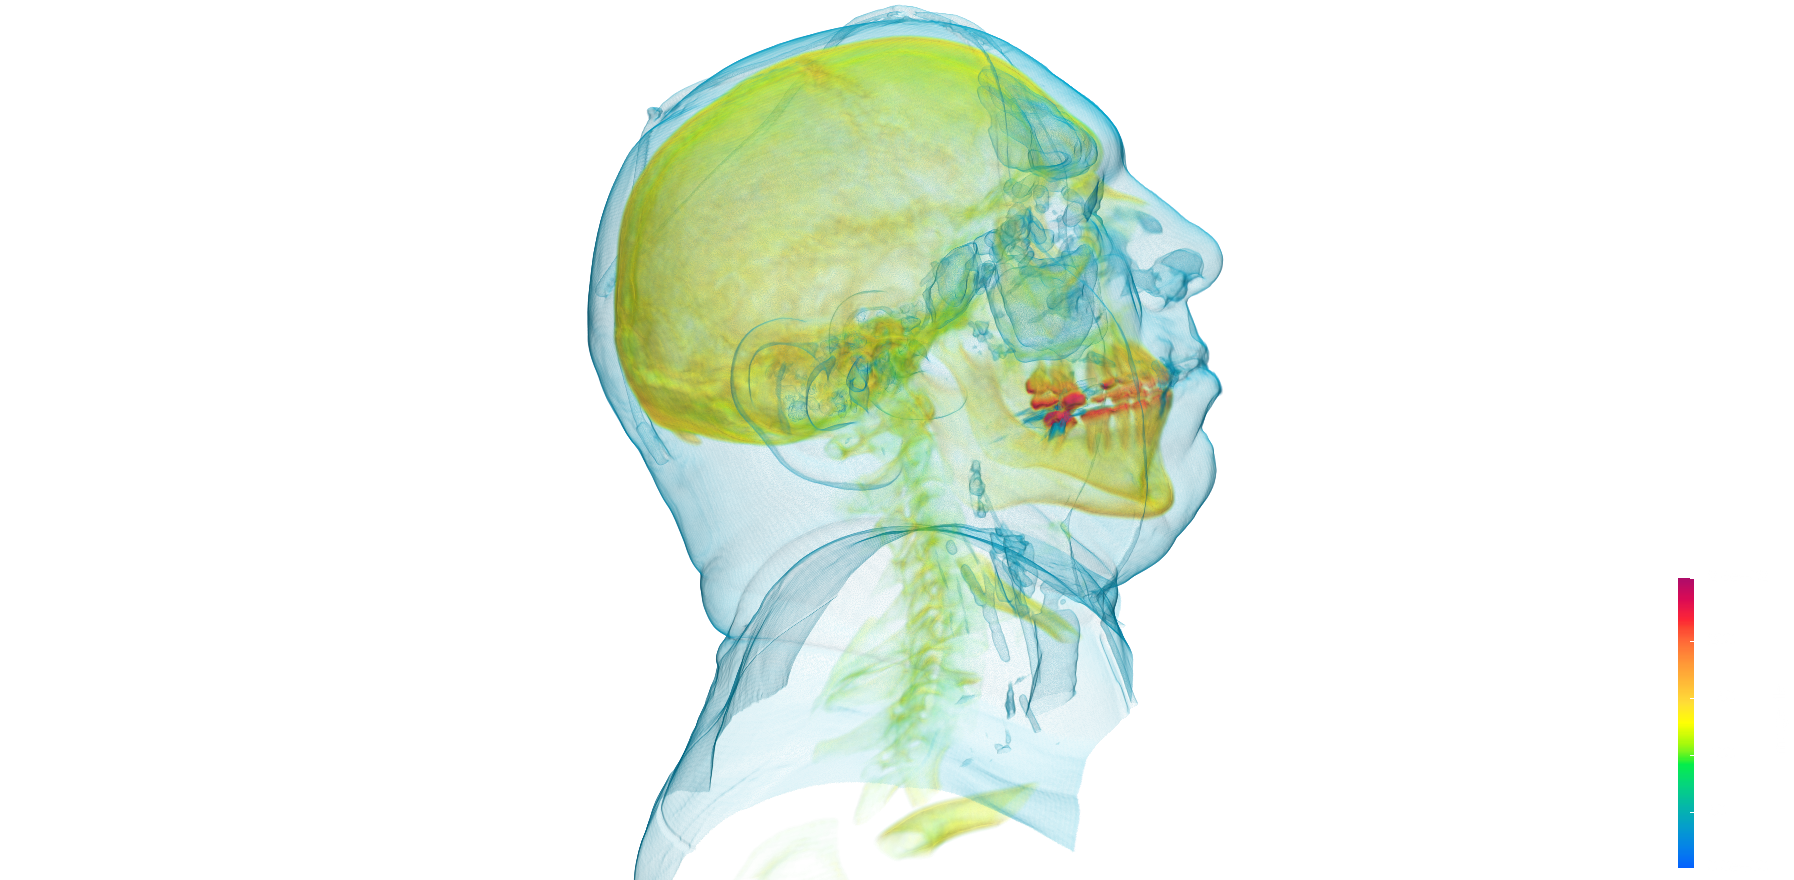
\includegraphics[width=\linewidth]{VisHuman_Head/human_head_2}
  \caption{Resulting visualisation}
\end{subfigure}
\caption{Visualising bones density}
\end{figure}

\subsection {Asian Dragon} 

The Asian Dragon is a \texttt{.ply} file containing a polygonal mesh consisting of 7219045 cells and 3609600 points of \texttt{float} type. The mesh is very dense, so that the surface looks fairly smooth. It requires a lot of zoom in order to see the components of the mesh.

\begin{figure}[h]
\centering
\begin{subfigure}{.5\textwidth}
  \centering
  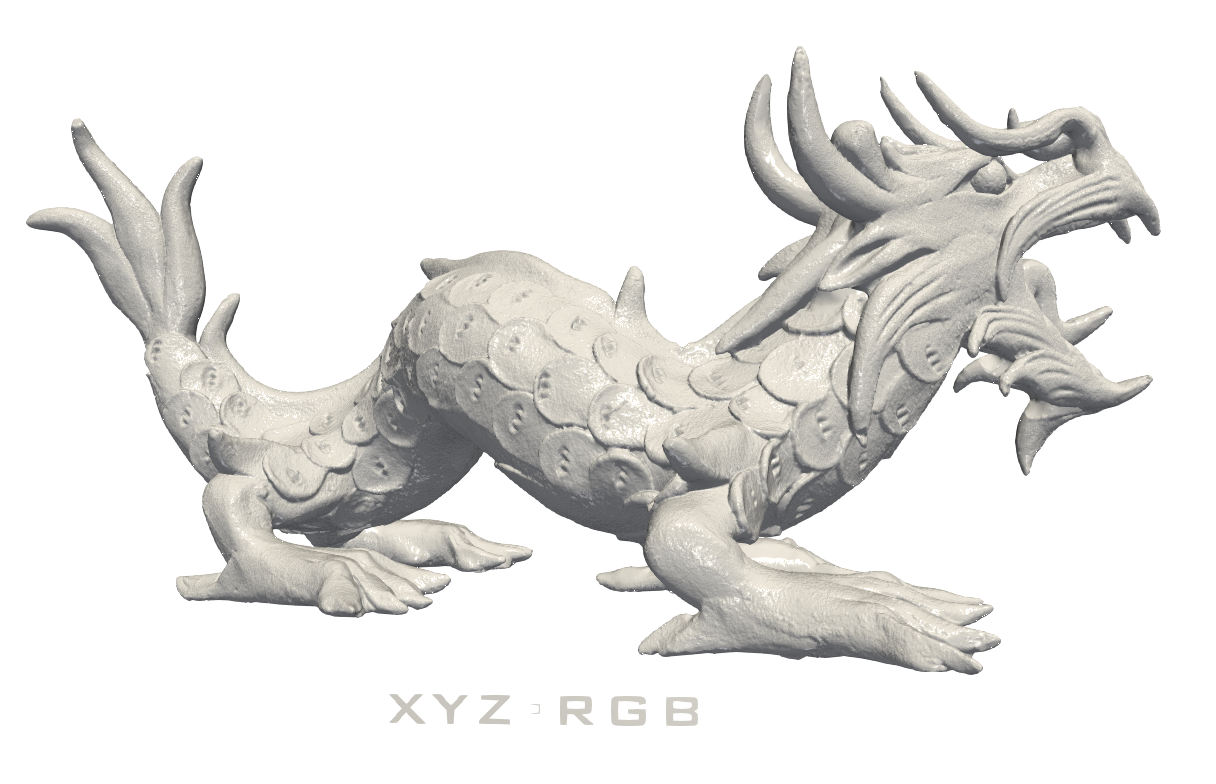
\includegraphics[width=\linewidth]{Asian_Dragon/asian_dragon}
  \caption{Entire dataset, visualised with \textit{surface}  \\
  representation, solid \texttt{\#ffffff} colour and 100\% \\ specular lightning}
\end{subfigure}%
\begin{subfigure}{.5\textwidth}
  \centering
  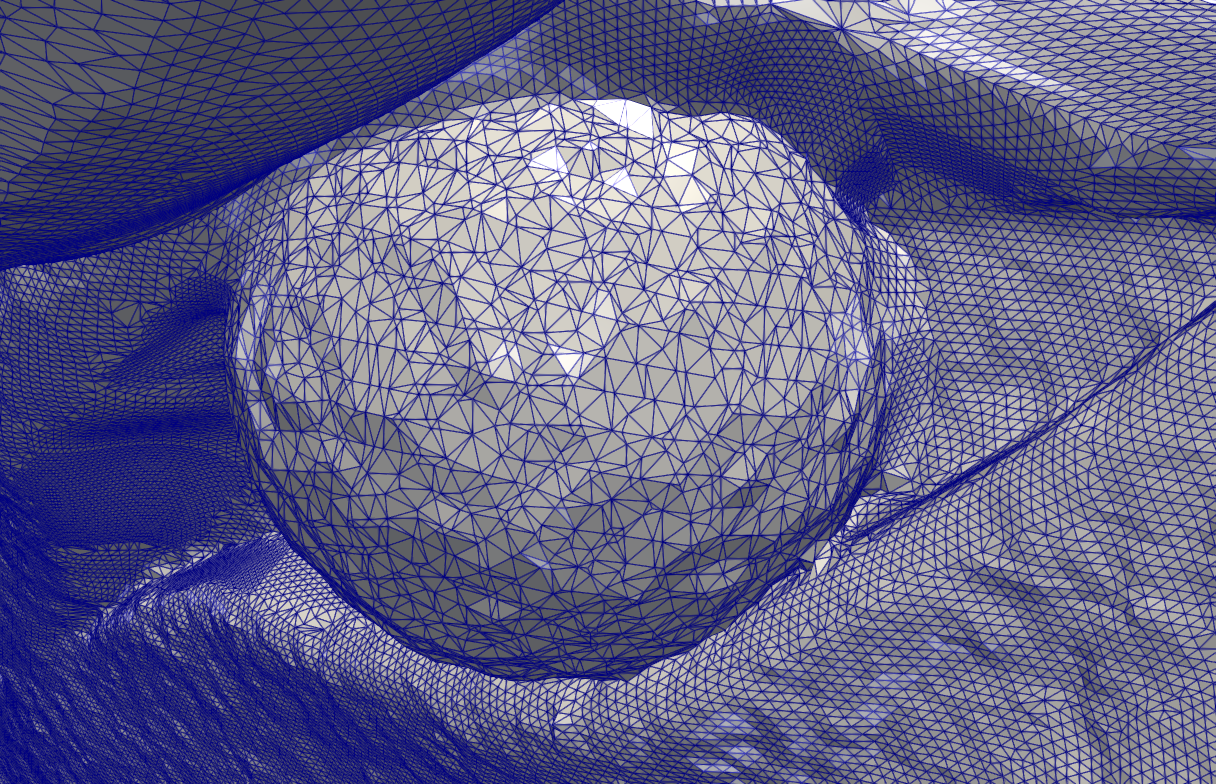
\includegraphics[width=\linewidth]{Asian_Dragon/eye_detail_edges}
  \caption{Eye detail to show the mesh, with \textit{surface with edges} representation, \texttt{\#000080} colour edges}
\end{subfigure}
\caption{Asian Dragon visualisation}
\end{figure}

\subsection {Particle tracing and streamlines}

For this task, we used a dataset from  \href{https://tuxriders.com/videos/postprocessing/}{TuxRiders}. 

For the particle tracing, we used a 2D simulation of a fluid flow in a tube. We produced an \href{https://imgur.com/a/Ge00wdk}{animation} where we combine a background with the evolution of the velocity over time and the movement of the particles. To help in distinguishing the traces left behind, each batch of particles has a different colour. We also extracted a single frame as an example, from the 70th timestep, but we decided to keep all the particles on the same colour, given the fact that it's a static image. 

For the streamlines, we see the behaviour of a fluid around a sphere. We decided to visualise the lines as tubes.

\begin{figure}[h]
\centering
\begin{subfigure}{.5\textwidth}
  \centering
  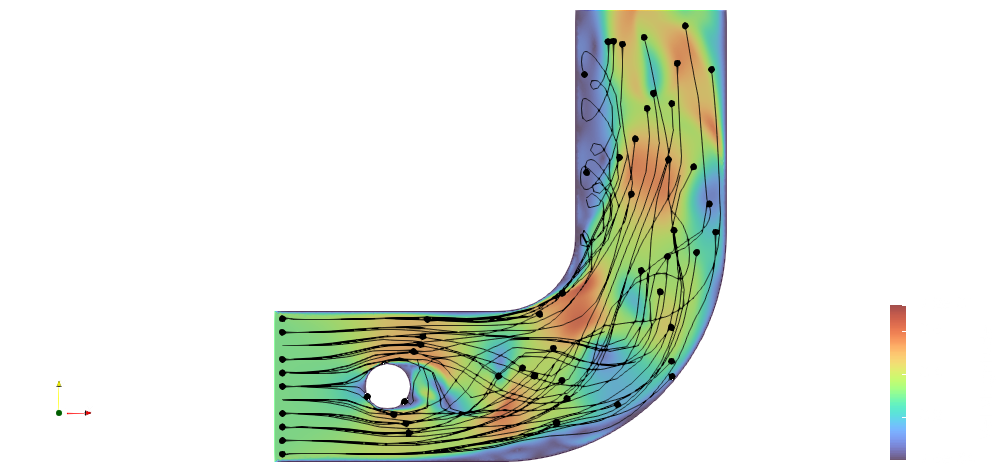
\includegraphics[width=\linewidth]{Fluid_Flow/particle_tracing}
  \caption{Particle tracing}
\end{subfigure}%
\begin{subfigure}{.5\textwidth}
\centering
  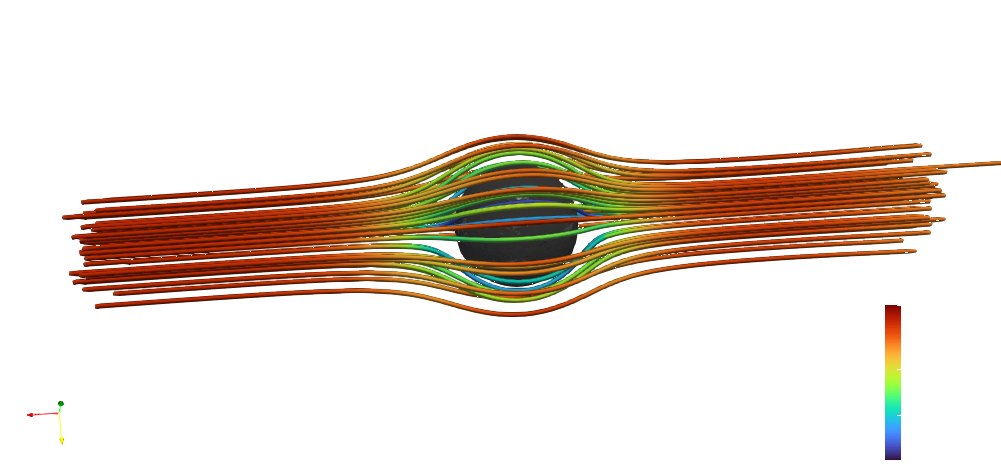
\includegraphics[width=\linewidth]{Fluid_Flow/stream_lines}
  \caption{Streamlines}
\end{subfigure}
\caption{}
\end{figure}

\subsection {RCSB protein data bank}

The RCSB protein data bank contains a lot of datasets for various proteins. Each dataset contains different information about the structure of a specific protein. We chose to visualise the \textit{1H59 insulin}. The closest 3D view visualisation can be achieved by using the \textit{NGL viewer} on the website, with the parameters shown in Figure \ref{insulin_el} and \ref{insulin_res}.

\begin{figure} [h!]
\centering
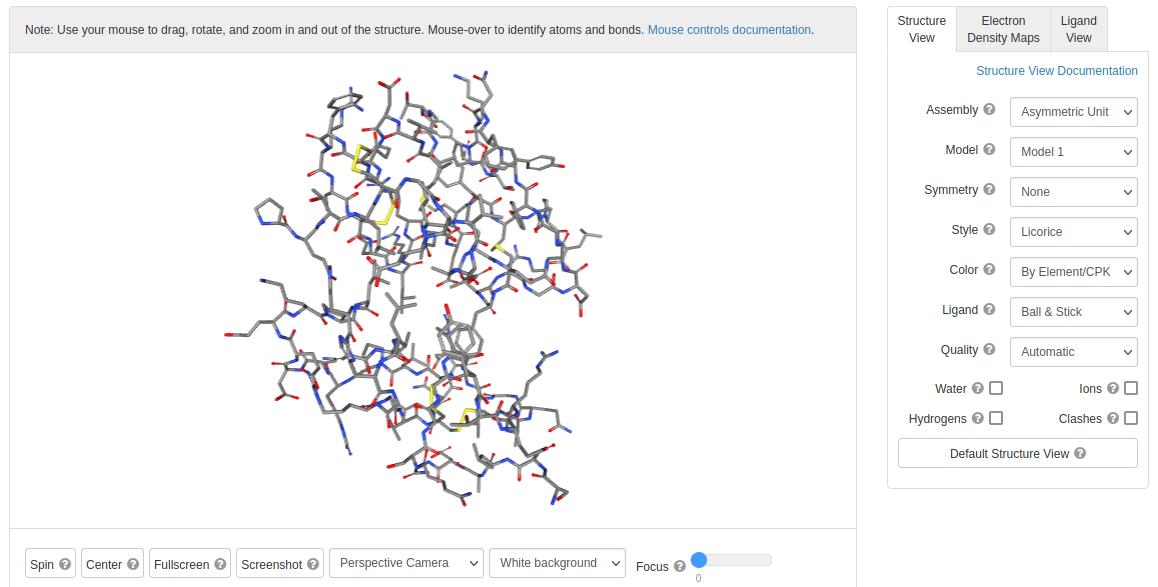
\includegraphics[width=0.8\linewidth]{Proteins/1h59_insulin_el}
\caption{1H59 insulin, element visualisation}
\label{insulin_el}
\end{figure}

\begin{figure} [h!]
\centering
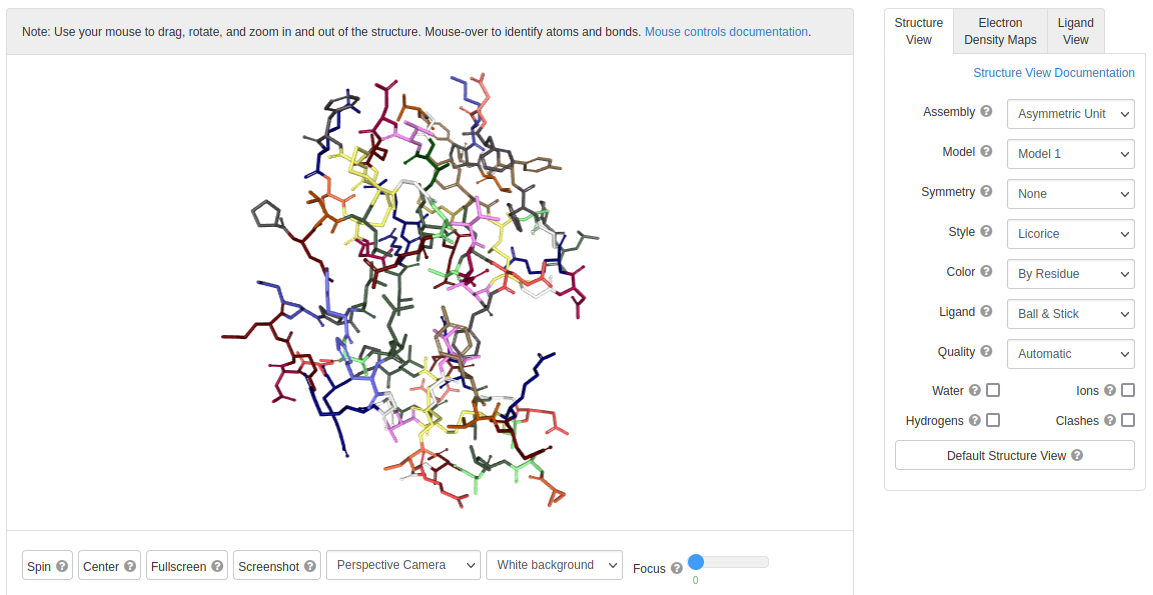
\includegraphics[width=0.8\linewidth]{Proteins/1h59_insulin_res}
\caption{1H59 insulin, residue visualisation}
\label{insulin_res}
\end{figure}

Very similar visualisations can be obtained in ParaView. 

For the one shown in Figure \ref{insulin_el}, we use the \textit{element} color property, the \textit{surface} representation and we specify in the color map editor to interpret values as categories. Then, we apply the \textit{BlueObeliskElements} preset.

For the one shown in Figure \ref{insulin_res}, we use the \textit{restype} color property, the \textit{surface} representation and we specify in the color map editor to interpret values as categories. Then, we apply the \textit{Brewer Qualitative Set3} preset.

\begin{figure}[h]
\centering
\begin{subfigure}{.5\textwidth}
  \centering
  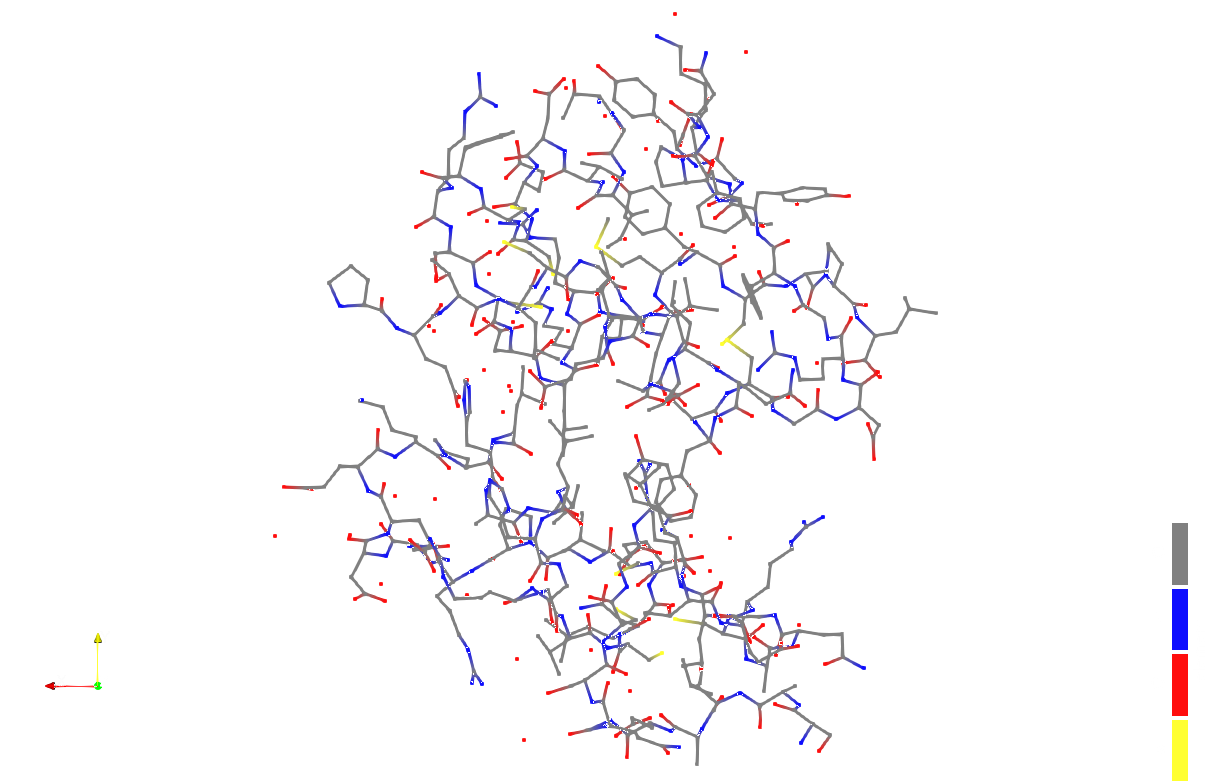
\includegraphics[width=\linewidth]{Proteins/1h59_insulin_el_pv}
  \caption{Element visualisation}
\end{subfigure}%
\begin{subfigure}{.5\textwidth}
\centering
  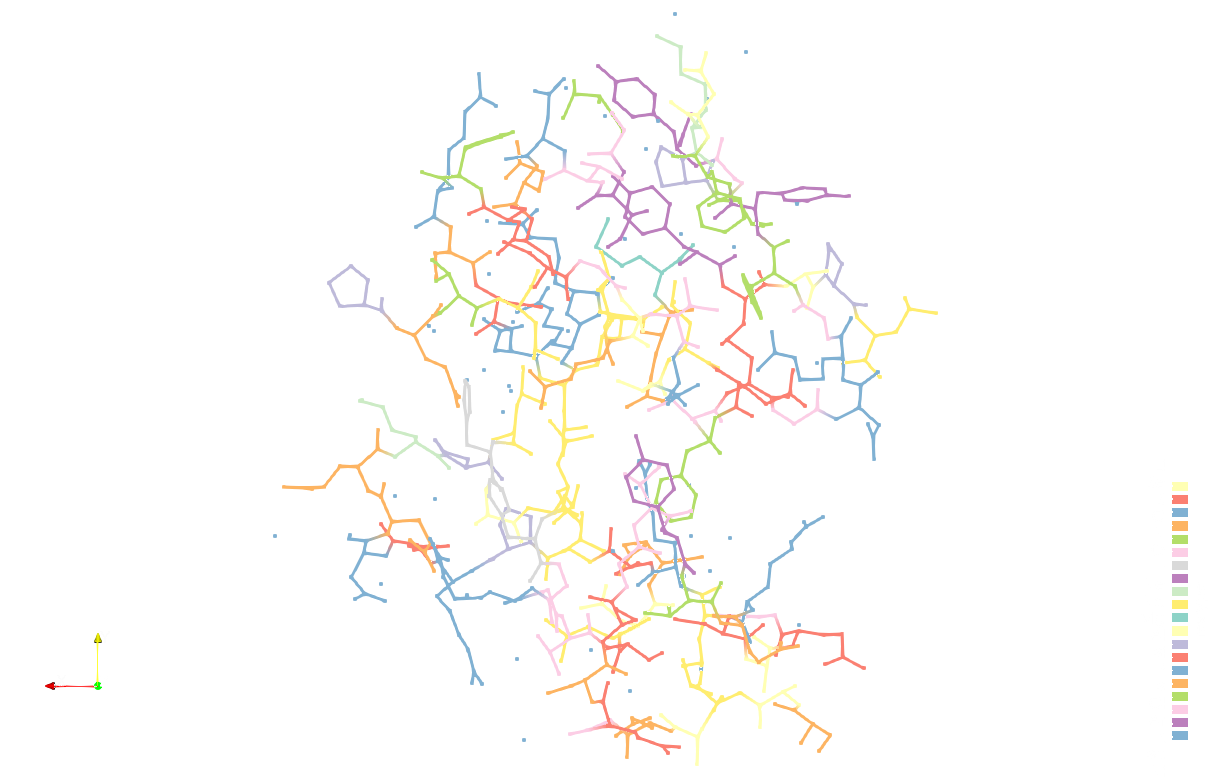
\includegraphics[width=\linewidth]{Proteins/1h59_insulin_res_pv}
  \caption{Residue visualisation}
\end{subfigure}
\caption{1H59 insulin in ParaView}
\end{figure}































\clearpage
%%%%%%%%%%%%%%%%%%%%%%%%%%%%%%%%%%%%%%%%%%%%
\section {Second part: Tableau}

In the second section we explore the default \textit{Superstore Sales} data set that comes with Tableau.

\subsection {Relation total sales - geographical position}







































\end{document}